\subsection{Some Detections of LIGO}

\subsubsection{GW190814}

Two advanced-LIGO detectors (Hanford, Washington and Livingston, Louisiana, USA) and the advanced-Virgo detector (Cascina, Italy), have detected gravitational waves from the inspiral and merger of a stellar-mass black hole and another compact object on 14th August, 2019 at 21:10:39 UTC. It has been named as GW190814 as the date suggests.

\begin{figure}[h]
    \centering
    \includegraphics[scale = 0.91]{images.tex/GW190814.jpg}
    \caption{Frequency Vs Time data of GW190814 in three observatories. Source:- \href{https://en.wikipedia.org/wiki/GW190814}{Wikipedia}}
\end{figure}

While the mass of one component of this binary could range from 22.2 to 24.3 $M_\odot$ black hole, the other component which was of 2.6 solar mass could be either a low-mass black hole or a heavy neutron star. The masses of the objects before merging differed by a factor of 9. This makes it the most extreme mass ratio known for some GW event. The source of this GW was in a small patch of sky of around 20 square degrees. Even after doing so much research, the counterpart of the black hole which was in the inspiral mechanism wasn’t observed. It can be that, either black hole consumed the neutron star completely or both were black holes. Had we observe an electromagnetic counterpart, which may not have happened due to a number of reasons, we could say the smaller object is mostly neutron star. 

\pagebreak

\subsubsection{GW170817}

On 17th August, 2017, LIGO and Virgo detectors observed a gravitational wave named as GW170817. It is known to be produced by two neutron stars merging into each other while spiralling closer and closer. The aftermath of this GW was observed by around 70 observatories on 7 continents as well as through space, across the electromagnetic spectrum, marking a significant breakthrough for multi-messenger astronomy. The discovery and subsequent observations of GW170817 got Breakthrough of the Year award for 2017 by the journal Science.

\begin{figure}[h]
    \centering
    \includegraphics[scale=0.78]{images.tex/GW170817_observatories.png}
    \caption{Frequency Vs Time data of GW170817 in three observatories. Source:- \href{https://en.wikipedia.org/wiki/GW170817}{Wikipedia}}
\end{figure}

The component masses of the binary are inferred to be between 1.17 and 1.60 $M_\odot$. After merging it makes the mass of about 2.74 $M_\odot$. The gravitational wave signal lasted for about 100 seconds. It started with a frequency of 24 $Hz$. It  inspiralled for around 3,000 cycles. The amplitude and frequency increased to a few hundred hertz as both the objects came nearer in the typical inspiral chirp pattern. Lastly, it ended with the collision at 12:41:04.4 UTC which was received as a signal in the interferometer. At first, it arrived at the Virgo detector in Italy. After 22 milliseconds, detectors at the LIGO-Livingston detector in Louisiana, United States got the signals. After another 3 milliseconds, the waves reached at the LIGO-Hanford detector in the state of Washington, United States. It was then compared with a prediction from the general theory of relativity given by Einstein to analyse it further. The source was localised within a sky region of 28\degree square which has a probability of 90\%.

A gamma-ray burst, GRB 170817A was detected. It lasted for $\approx$ 2 seconds. It was detected by Fermi and INTEGRAL spacecrafts. This bursts began at 1.7 seconds after the signal received denoting the merge of the objects. It's a hypothesis that neutron star mergers cause gamma-ray bursts which gets confirmed with this merger.

\pagebreak

\subsubsection{GW190521}

LIGO-VIRGO detectors detected a short signal from a binary black hole merger
on May 21,2019 at 03:02:29 UTC. The event occurred at a luminosity distance $5.3_{-2.6}^{+2.4}\,Gpc$ with a red shift of $0.82_{-0.34}^{+0.28}$. The signal lasted for about 0.1 seconds long and had a peak frequency of about $60\,Hz$. Since the time period and frequency is inversely proportional to the binary’s total mass, and since the signal was so short, this could imply that in this event the most massive black holes could have collided when compared to the collisions detected so far with a total mass of $150_{-17}^{+29}\,M_\odot$. The two black holes weighed upto $85_{-14}^{+21}\, M_\odot$ and $66_{-18}^{+17} \,M_\odot$ giving rise to a $142_{-16}^{+28}\, M_\odot$ remnant black hole. \cite{GW190521_1}

\begin{figure}[h]
    \centering
    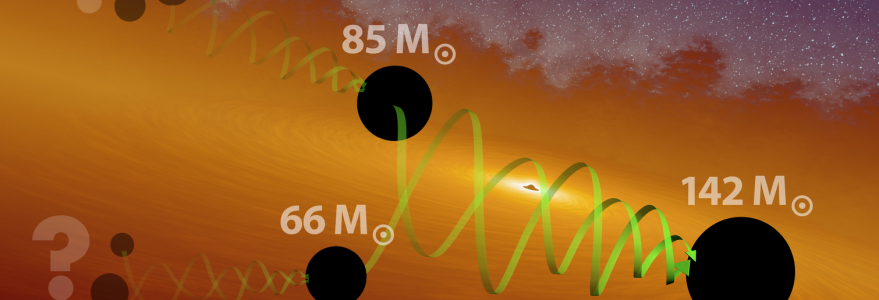
\includegraphics[scale = 0.5]{images.tex/GW190521 representation.jpg}
    \caption{Pictorial representation of GW190521 merger. Source :- \href{https://en.uw.edu.pl/virgo-and-ligo-unveil-new-and-unexpected-black-hole-populations/}{en.uw.edu.pl}}
\end{figure}

The mass of the remnant black hole is between 100 and 1000 $M_\odot$, making it the first intermediate mass black hole to be detected. Not only is the remnant black hole bizarre, but the two mergers had masses which are impossible to be directly formed by collapsing stars. This led to the theory that these kinds of black holes may be formed by merging of smaller black holes or stars can form black holes with higher masses. Regions like the galactic centre or star clusters might favour the existence of such black holes \cite{GW190521_2}. An electromagnetic counterpart was also detected but its association with the event GW190521 is uncertain. This is the first time an electromagnetic counterpart has ever been detected from the merging of black holes. The one unsolved problem here is why an electromagnetic counterpart observed as the black hole mergers do not emit light. It is approximated that the two black holes orbited a super massive black hole. After the formation of the intermediate mass black hole, it must have crossed the gaseous disk, that caused it to light up. The first largest merger and the unexplained electromagnetic counterpart are some of the most notable features.


\begin{figure}[h]
    \centering
    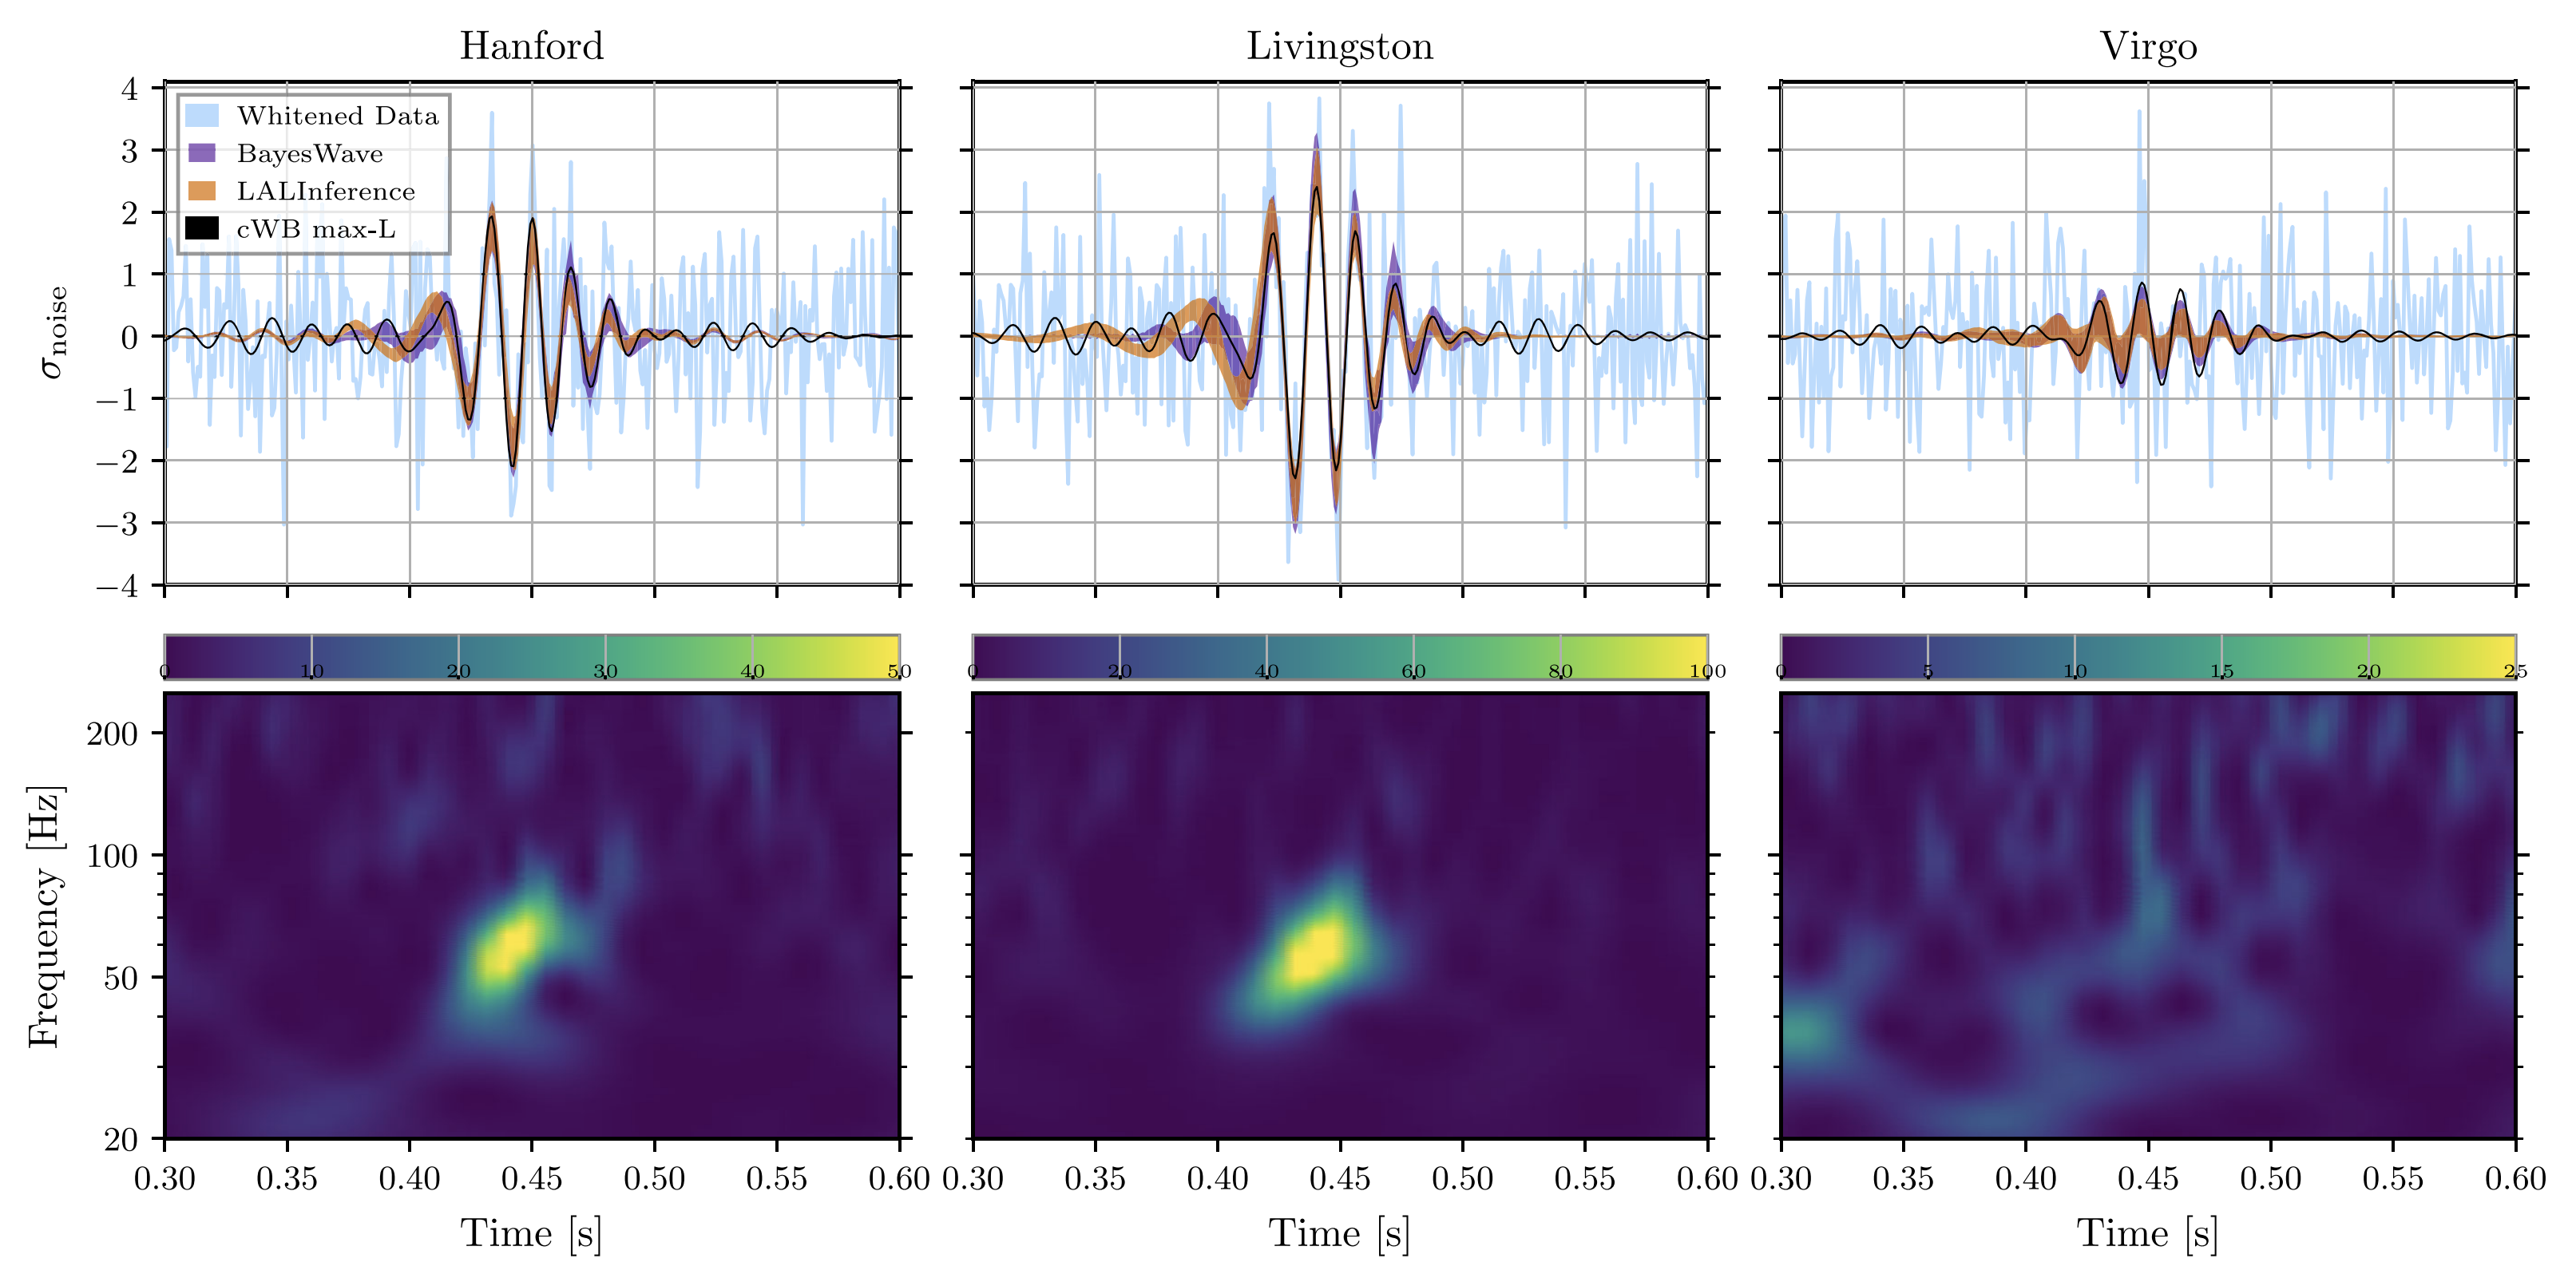
\includegraphics[width=15cm, height = 8cm]{images.tex/GW190521.png}
    \caption{Wave form of GW190521 signal. \\ Source :- \href{https://journals.aps.org/prl/abstract/10.1103/PhysRevLett.125.101102}{GW190521:A Binary Black Hole Merger with a Total Mass of 150$M_\odot$}}
\end{figure}

\pagebreak

\subsubsection{GW190425}
The signal was detected by LIGO-Livingston and VIRGO detector during the third observational run O3 on 25 April,2019 at 08:18:05 UTC whereas LIGO-Hanford was temporarily offline.The signal originated from a region of the sky which was not in plain sight for VIRGO and it lied just above the detection threshold for LIGO-Livingston. Luminosity distance of the event was 159$_{-71}^{+69}$ Mpc. \cite{GW190425_1}

\begin{figure}[htpb]
    \centering
    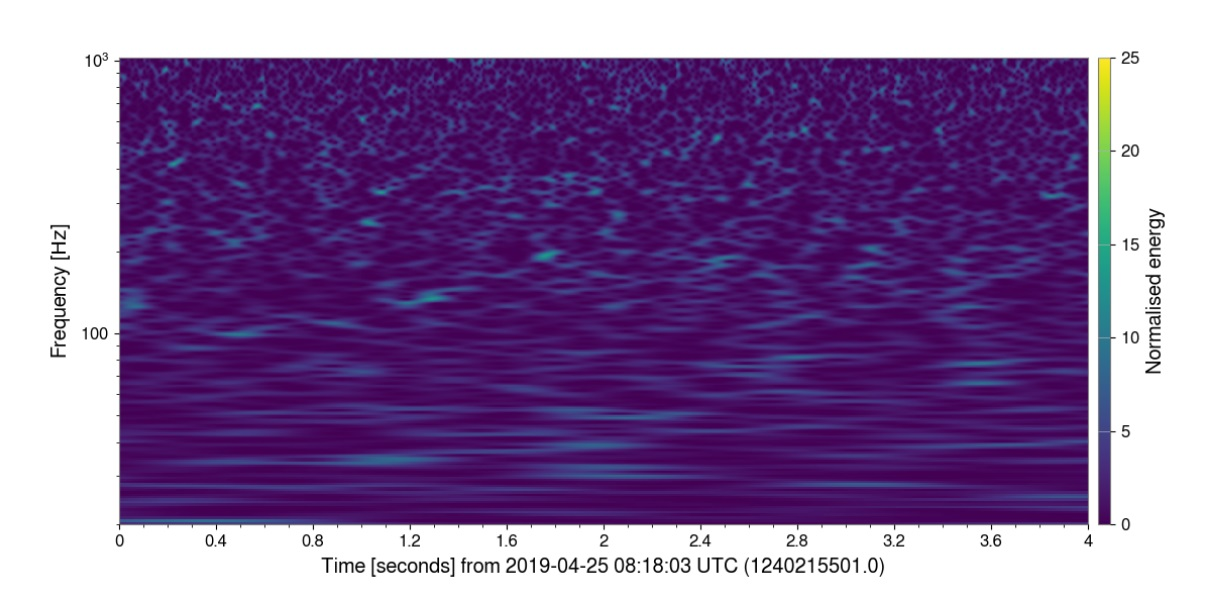
\includegraphics[scale=0.75]{images.tex/GW190425 L1.jpg}
    \caption{Signal detected by L1. Source :- \href{https://www.gw-openscience.org/eventapi/html/O3_Discovery_Papers/GW190425/v1/}{gw-openscience.org}}
    \end{figure}
    
\begin{figure}[htpb]
    \centering
    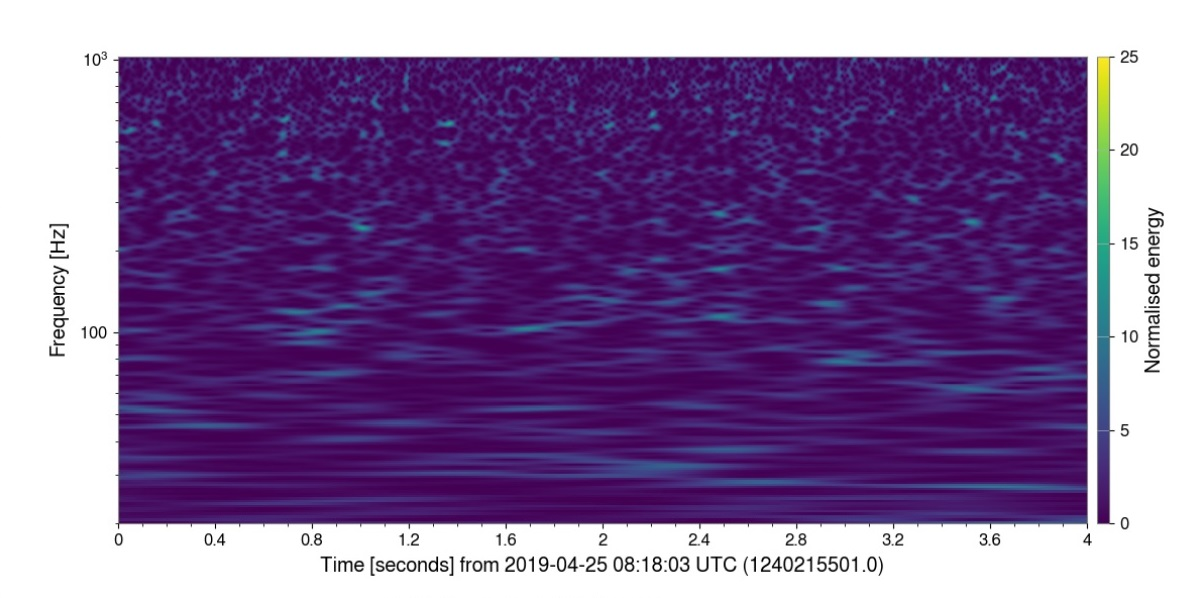
\includegraphics[scale=0.75]{images.tex/GW190425 V1.jpg}
    \caption{Signal detected by V1. Source :- \href{https://www.gw-openscience.org/eventapi/html/O3_Discovery_Papers/GW190425/v1/}{gw-openscience.org}}
\end{figure}

The mass of the mergers was estimated to be $1.61-2.52\,M_\odot$ and $1.12 - 1.68\,M_\odot$.The total mass of the compact binary was $3.4_{-0.1}^{+0.3}\, M_\odot$, greater than any known binary neutron stars. This suggests that the formation of GW190425 was different than the known binary neutron stars. One possible explanation for this is that the source consisted of a neutron star and a $4.5\,M_\odot$ helium star which evolved to form an eccentric double neutron star \cite{Romero_Shaw_2020}. Unlike the other neutron star mergers that produced electromagnetic counterparts, no such counterparts were observed for GW190425 \cite{GW190425_1}.

\pagebreak

\subsubsection{GW190412}

While the inferred individual masses of the coalescing black holes (BHs) are each within the range of masses that have been observed before, previously detected binaries all had mass ratios $ q = \frac{m_2}{m_1}$ (with $m_1 \geq m_2$) that were according to unity. GW190412, is the first observation of Gravitational waves by LIGO from a coalescing binary with indubitably unequal masses. GWs from this event carry faint but clearly measurable evidence of radiation that oscillates at frequencies with subdominant contributions for the first time as a result of the mass asymmetry of the BBH system.

\begin{figure}[h]
    \centering
    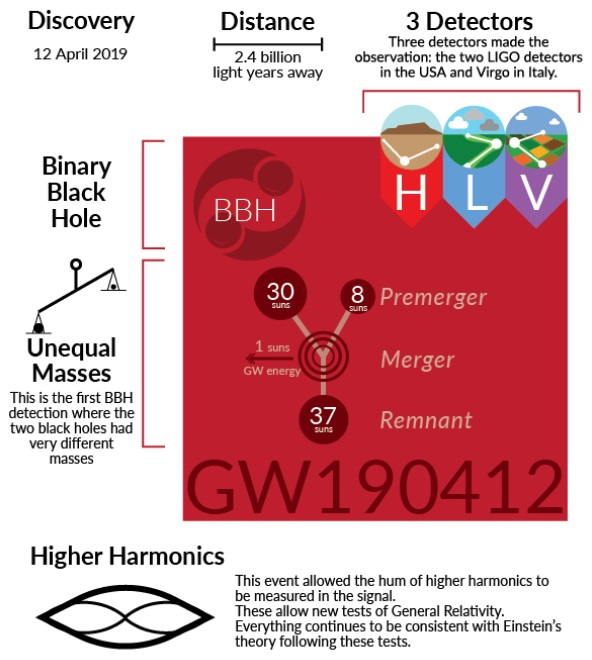
\includegraphics[scale=1.15]{images.tex/GW190412.jpg}
    \caption{Characteristics of GW190412. Source :- \href{https://www.ligo-india.in/outreach/detections/gw190412/}{LIGO-India.in}}
\end{figure}

Einstein’s Theory of General Relativity predicts that although gravitational radiation from compact binaries is dominated by a quadrupolar structure, it also contains weaker contributions from subdominant multi poles. In particular, gravitational radiation from systems with significantly asymmetric component masses consist of stronger contributions from higher multi poles. GW190412 presents strong evidence for contribution to gravitational radiation beyond the leading quadrupolar order in asymmetric systems.

\pagebreak

\subsubsection{GW170104}

GW170104, a gravitational-wave signal produced by the coalescence of a pair of stellar-mass black holes, was measured on 4th of January 2017 at 10:11:58.6 UTC by the Hanford and Livingston advanced detectors of the Laser Interferometer Gravitational-Wave Observatory with a network signal-to-noise ratio of 13 and a false alarm rate less than 1 in 70 000 years. The inferred component black hole masses are $31.2^{+8.4}_{-6.0}\,M\odot$  and $19.4^{+5.3}_{-5.9}\,M\odot$ (with 90\% credibility). The gravitational wave frequency at peak GW strain was $160$ to $199\, Hz$. \cite{PhysRevLett.118.221101}

\begin{figure}[h]
    \centering
    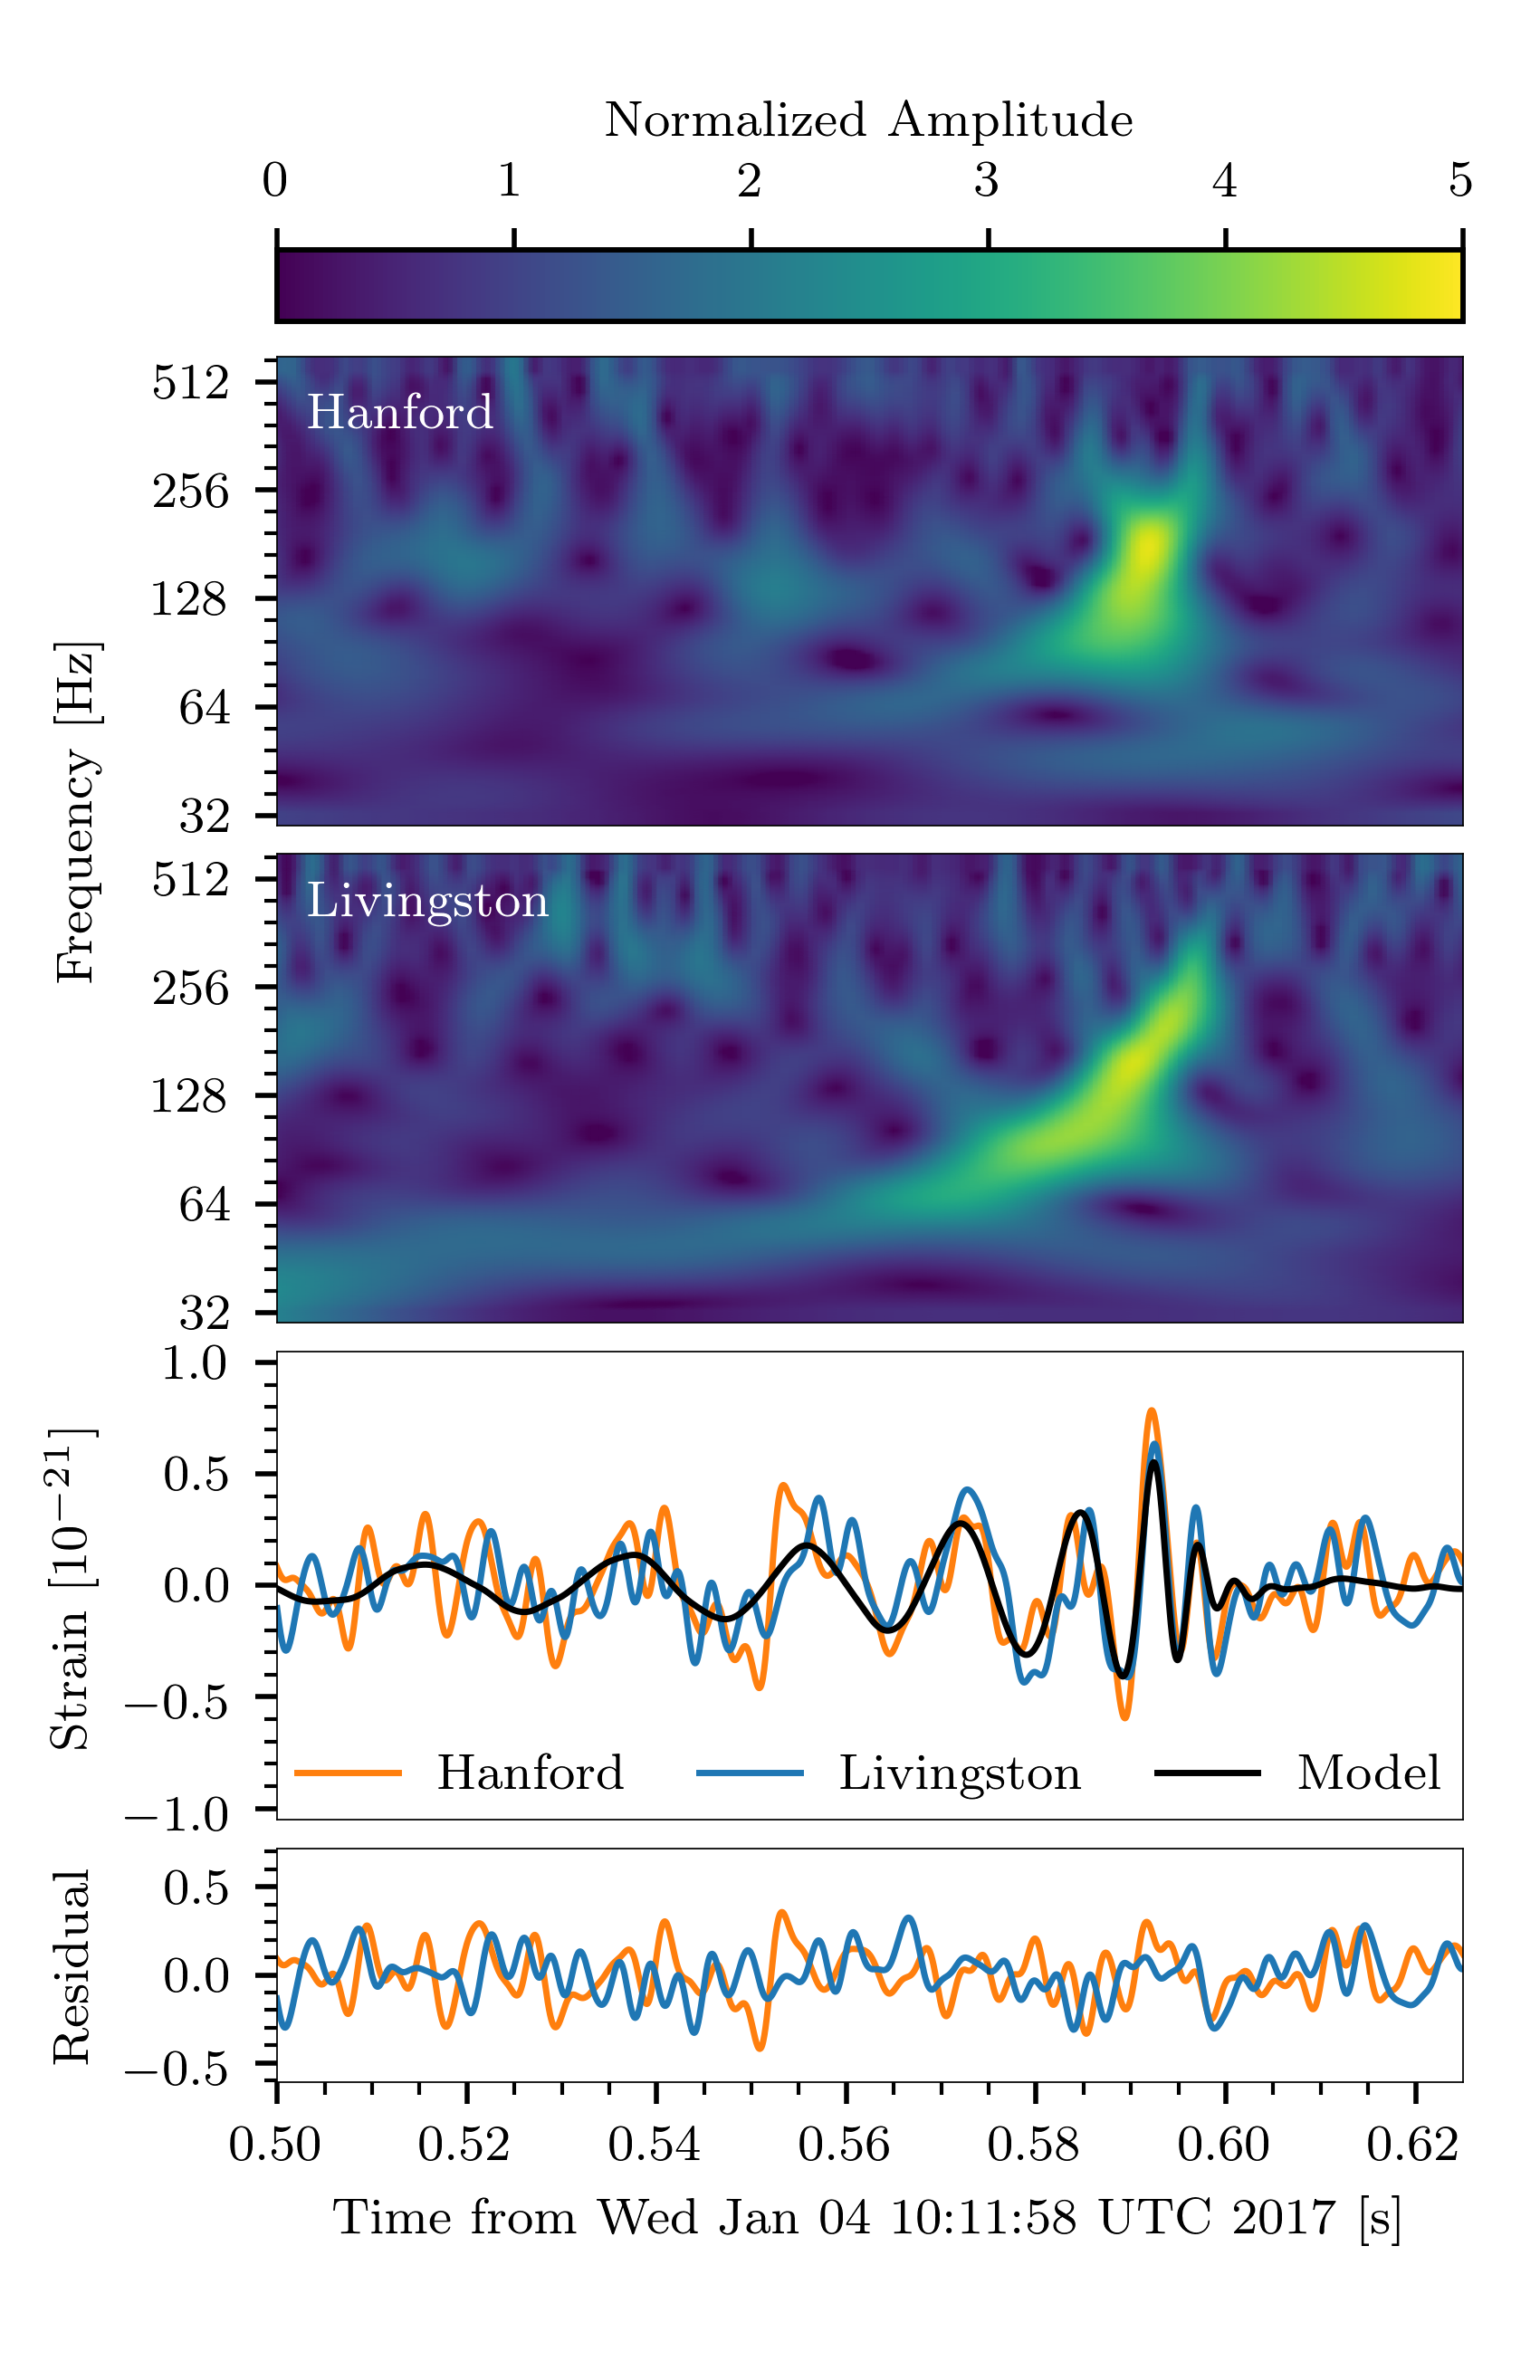
\includegraphics[scale=1.2]{images.tex/GW170104.png}
    \caption{Signal of GW170104 merger. Source :- \href{https://www.ligo.org/science/Publication-GW170104/}{LIGO.org}}
\end{figure}

Analyzing GW170104 signal yielded a new upper bound on the mass of gravitons assuming they are dispersed in vacuum like massive particles. This upper bound is equal to $7.7\times10^{-23} \, eV/c^2$. The spin axes of the black holes were unlikely to be aligned with the axis of the binary orbit. This hints that the binary black hole system was formed dynamically in a dense star cluster as an outcome of gravitational interaction between stars and binary stars, where randomly aligned spin axes are expected. The alternative scenario suggests that the system was formed out of a binary star system consisting of two main sequence stars. Although not entirely ruled out, this scenario is not favoured because black holes formed in such a binary are more likely to have positively aligned spins.

\pagebreak
